%\documentclass[8pt, handout]{beamer}
%\usepackage{pgfpages} 								%Для распечатки
%\pgfpagesuselayout{2 on 1}[a4paper,border shrink=10mm]

\documentclass[8pt]{beamer}

\usepackage[english,russian]{babel}
\usepackage[utf8]{inputenc}
\usepackage{mflogo}
\usepackage{amsmath,amsfonts,amssymb}
\usepackage{euscript}
\usepackage{graphicx}
\usepackage{xcolor}
\usepackage{transparent}



\beamertemplatenavigationsymbolsempty

\usetheme{EastLansing}
\setbeamercovered{transparent}


\title[Дифференциальное исчисление]{Математический анализ\\ Тема 3: Дифференциальное исчисление}
\author[Выборный Е. В.]{Выборный Евгений Викторович\\ email: evybornyi@hse.ru}
\date{Москва 2015} 


\makeatletter
\setbeamertemplate{footline}{
    \leavevmode%
    \hbox{%
    \begin{beamercolorbox}[wd=.25\paperwidth, ht=2.5ex, dp=1ex, center]{author in head/foot}%
        \usebeamerfont{author in head/foot}%
        \insertshortauthor
    \end{beamercolorbox}%
    \begin{beamercolorbox}[wd=.5\paperwidth,ht=2.5ex,dp=1ex,center]{title in head/foot}%
        \usebeamerfont{title in head/foot}\insertshorttitle
    \end{beamercolorbox}%
    \begin{beamercolorbox}[wd=.25\paperwidth,ht=2.5ex,dp=1ex,right]{date in head/foot}%
        \usebeamerfont{date in head/foot}\insertshortdate{}\hspace*{2em}
        \insertframenumber{} / \inserttotalframenumber\hspace*{2ex}
    \end{beamercolorbox}}%
    \vskip0pt%
}
\makeatother

\makeatletter
\setbeamertemplate{title page}
{
\centering
 \usebeamerfont{author}\insertauthor
 \vfill
 \begin{beamercolorbox}[rounded=true,shadow=true,sep=8pt,center]{title}
  \usebeamerfont{title}\inserttitle
 \end{beamercolorbox}
\vfill
\centering
\insertdate\par
 \vskip0.2em
}
\makeatother

\begin{document}
%\parindent=1.5em %красная строка

\begin{frame}
\titlepage
\end{frame}

\begin{frame}{Дифференциал и производная функции}
Пусть функция $f(x)$ определена в некоторой окрестности точки $x_0$.
\begin{block}{Определение (Дифференциал)}
Функция $f(x)$ называется {\bf дифференцируемой} в точке $x_0$, если ее приращение можно представить в виде
$$f(x_0+\Delta x) - f(x_0) = A\cdot \Delta x + o(\Delta x)\quad (\Delta x\to0).$$
Линейная часть приращения (как функция от $\Delta x$) называется {\bf дифференциалом функции} $f(x)$ в точке $x_0$. Пишут
$$df(x_0)=df(x_0)(\Delta x) = A\cdot \Delta x\quad \forall\ \Delta x\in\mathbb{R}.$$
\end{block}
\vskip-1em
\begin{block}{Определение (Производная)}
Пусть функция $f(x)$ дифференцируема в точке $x_0$. Тогда соответствующее число $A$ называют {\bf производной} функции $f(x)$ в точке $x_0$. Пишут
$$A=f'(x_0).$$
\end{block}
\vskip-1em
Таким образом,
$$f(x_0+\Delta x) - f(x_0) = f'(x_0)\cdot \Delta x+o(\Delta x)\quad (\Delta x\to0).$$
\end{frame}

\begin{frame}{Дифференциал и производная функции}
Пусть функция $f(x)$ дифференцируема в точке $x_0$. Тогда
$$f(x_0+\Delta x) - f(x_0) = f'(x_0)\cdot \Delta x+o(\Delta x)\quad (\Delta x\to0).$$
Поделив на $\Delta x$, получаем
$$f'(x_0) = \frac{f(x_0+\Delta x) - f(x_0)}{\Delta x} + o(1)\quad (\Delta x\to0).$$
Устремляя $\Delta x\to0$, получаем, что
$$f'(x_0) = \lim_{\Delta x\to 0} \frac{f(x_0+\Delta x) - f(x_0)}{\Delta x}.$$
Эту формулу часто используют для определения и вычисления производных. Мы доказали, что этот предел (производная $f'(x_0)$) существует, если функция $f(x)$ дифференцируема в точке $x_0$. Верно и обратное утверждение {\bf (проверьте дома)}. Таким образом, мы доказали следующую теорему.
\begin{block}{Теорема (2-ое определение производной)}
Функция $f(x)$, определенная в некоторой окрестности $x_0$, является дифференцируемой в точке $x_0$ тогда и только тогда, когда существует конечный предел
$$f'(x_0) = \lim_{\Delta x\to 0} \frac{f(x_0+\Delta x) - f(x_0)}{\Delta x}.$$
\end{block}
\end{frame}

\begin{frame}{Примеры вычисления дифференциала и производной}
\begin{enumerate}
\item Пусть $y(x)=x$. Тогда
$$y(x+\Delta x) - y(x) =(x+\Delta x) - x = \Delta x = 1\cdot \Delta x.$$
Следовательно, функция $y(x)=x$ дифференцируема в любой точке $x$, ее дифференциал и производная соответственно равны:
$$dy(x) = dx = 1\cdot \Delta x, \qquad y'(x) = 1.$$
\item Пусть $y(x)=x^2$. Тогда
$$y(x+\Delta x) - y(x) = (x+\Delta x)^2 - x^2 = 2 x \Delta x +\left(\Delta x\right)^2.$$
Поскольку $\left(\Delta x\right)^2=o(\Delta x)$ при $\Delta x\to0$, то
$$y(x+\Delta x) - y(x) =  2 x \Delta x +o(\Delta x),\quad \Delta x\to0.$$
Следовательно, функция $y(x)=x^2$ дифференцируема в любой точке $x$, ее дифференциал и производная соответственно равны:
$$dy(x) = dx^2 = 2 x \Delta x=2x\ dx, \qquad y'(x) = 2x.$$
\end{enumerate}
\end{frame}

\begin{frame}{Замечания касательно обозначений}
Пусть $f(x)$ --- дифференцируемая в точке $x_0$ функция, а $df(x_0)$ --- соответствующий дифференциал. Тогда
$$df(x_0) = f'(x_0) d x,$$
 где равенство необходимо понимать как тождество двух функций от $\Delta x$, справедливое при любых $\Delta x\in\mathbb{R}$. Следовательно,
$$f'(x_0) = \frac{df(x_0)}{dx}.$$
Важно понимать, что дифференциал функции $f$ --- это $df$, а $df(x_0)$ --- это значение дифференциала $df$ в точке $x_0$, а не дифференциал выражения $f(x_0)$:
$$df(x_0)\ne d\left( f(x_0) \right).$$
 Во избежание путаницы в обозначениях часто пишут, что
 $$df(x_0) = (df)(x_0) = d\left(f(x)\right)\Big|_{x=x_0},$$
где символ $\Big|$ означает подстановку. Соответственно, для производной используют следующие обозначения:
$$f'(x_0) =\left( f(x) \right)'\Big|_{x=x_0} = \frac{df(x_0)}{dx} = \frac{df}{dx}(x_0) = \frac{df(x)}{dx}\Big|_{x=x_0}.$$
\end{frame}

\begin{frame}{Геометрический смысл производной и дифференциала}
По определению функция $f$ дифференцируема в точке $x_0$, если
$$f(x) = f(x_0) + f'(x_0)(x - x_0)+o(x-x_0)\quad x\to x_0,$$
то есть значение функции $f$ в точке $x$, близкой к $x_0$, можно приблизить значением линейной функции 
$$y(x)= f(x_0) + f'(x_0)(x - x_0)$$
 с небольшой погрешностью $o(x-x_0)$.
 
 \begin{block}{Определение (Касательная)}
Линейную функцию $y(x)= f(x_0) + f'(x_0)(x - x_0)$  называют {\bf касательной} к функции $f(x)$ в точке $x_0$, а соответствующую прямую на графике --- касательной к графику функции $f(x)$ в точке $x_0$.
 \end{block}
\begin{center}
 \vskip-1em
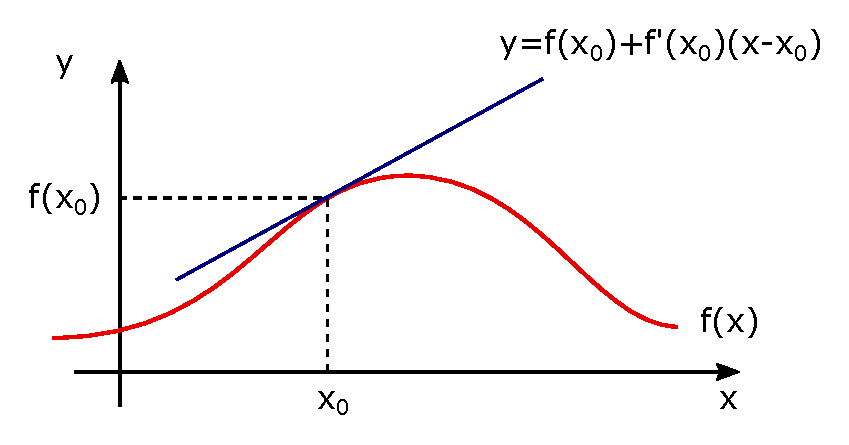
\includegraphics[scale=0.5]{kos.pdf}
\end{center}
\end{frame}

\begin{frame}{Геометрический смысл производной и дифференциала}
\begin{block}{Касательная как предел секущих}
Рассмотрим секущую $y_{\text{сек.}}$, которая пересекает график функции $f$ в точках $x_0$ и $x_0+\Delta x$. Тогда уравнение этой секущей будет иметь вид:
$$y_{\text{сек.}}=f(x_0)+\frac{f(x_0+\Delta x)-f(x_0)}{\Delta x}(x-x_0).$$
Если функция $f(x)$ дифференцируема в точке $x_0$, то для любого фиксированного $x$ будет существовать предел $y_{\text{сек.}}$ при $\Delta x\to0$. Очевидно, что эта секущая переходит в касательную в пределе при $\Delta x\to0$.
\end{block}
\begin{block}{Физический смысл производной}
Пусть материальная точка движется прямолинейно и равномерно. Тогда ее скорость $v$ определяется, как отношение пройденного пути $s$ к затраченному времени $t$: $v = s/t$.
Если положение точки описать функцией $x=x(t)$, то
$$v=\frac{x(t_1)-x(t_0)}{t_1-t_0}.$$
Если движение является неравномерным, то выражение для скорости $v$ является функцией от $t_0$ и $t_1$. Данное число называют средней скоростью $v_{\text{средн.}}$ на интервале $(t_0,t_1)$. Мгновенной скоростью $v=v(t_0)$ при $t=t_0$ называют предел величины $v_{\text{средн.}}$ при $t_1\to t_0$.
\end{block}
\end{frame}

\begin{frame}{Производные основных функций}
\begin{enumerate}
\item Пусть $f(x) = C$ --- константа, не зависящая от $x$. Тогда
$$\left( C \right)' = \lim_{\Delta x\to0}\frac{C - C}{\Delta x} =0.$$
\item Пусть $f(x) = x^{\alpha}$, $x>0$, $\alpha\ne0$. Тогда
$$\left( x^{\alpha} \right)' = \lim_{\Delta x\to0}\frac{(x+\Delta x)^{\alpha} - x^{\alpha}}{\Delta x} = x^\alpha  \lim_{\Delta x\to0}\frac{(1+\Delta x/x)^{\alpha} - 1}{\Delta x} =  x^\alpha  \lim_{\Delta x\to0}\frac{\alpha \ \Delta x / x}{\Delta x} = \alpha\ x^{\alpha-1}.$$
Если $\alpha$ --- целое, то это правило сохраняется для всех $x\in\mathbb{R}$.
\item Пусть $f(x)=\sin(x)$. Тогда
$$\left( \sin(x) \right)' =
 \lim_{\Delta x\to0} \frac{\sin(x+\Delta x) - \sin(x)}{\Delta x} =
 \lim_{\Delta x\to0} \frac{2\sin(\Delta x/2)\cos(x+\Delta x/2)}{\Delta x}=
$$
$$=
 \lim_{\Delta x\to0} \frac{\sin(\Delta x/2)}{\Delta x/2}\cdot
 \lim_{\Delta x\to0} \cos(x+\Delta x/2)=1\cdot\cos(x)=\cos(x).
$$
\item Пусть $f(x)=e^x$. Тогда
$$\left( e^x \right)' =
 \lim_{\Delta x\to0} \frac{e^{x+\Delta x} -e^x}{\Delta x} =
e^x \lim_{\Delta x\to0} \frac{e^{\Delta x}-1}{\Delta x}=e^x\cdot 1=e^x.
$$
\end{enumerate}
\end{frame}

\begin{frame}{Производные основных функций}
Аналогичным образом можно получить следующую таблицу производных:
\begin{center}
\vskip-0.5em
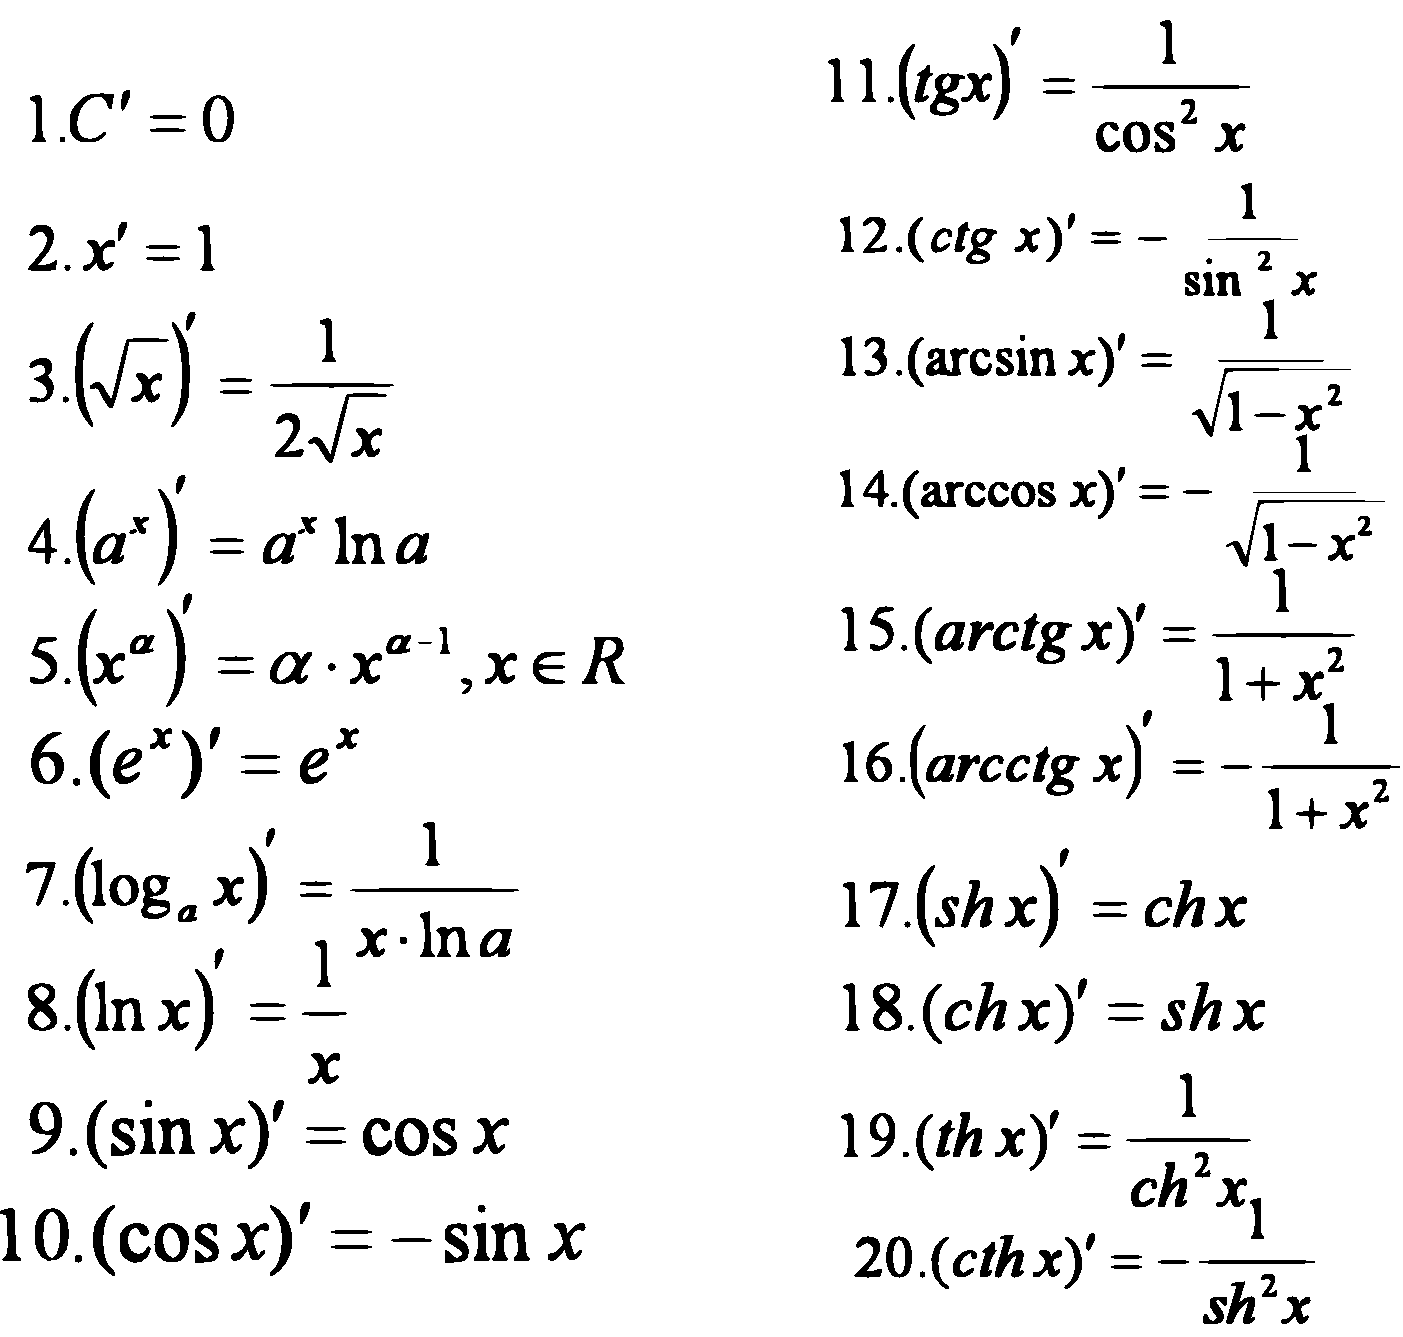
\includegraphics[scale=0.3]{table.pdf}
\end{center}
\vskip-0.5em
Проведите вычисления производных для всех функций из таблицы!
\end{frame}

\begin{frame}{Правила дифференцирования}
Свойства производной и правила дифференцирования:
\begin{enumerate}
\item Если производная $f'(x_0)$ существует, то она определена однозначно.
\vskip0.5em
{\bf Доказательство.} Данное свойство следует из свойств предела.

\item Если функция $f$ дифференцируема в точке $x_0$, то она непрерывна в этой точке.
\vskip0.5em
{\bf Доказательство.} Дано: 
$$f(x)-f(x_0) = f'(x_0)(x-x_0)+o(x-x_0)\quad \text{при } x\to x_0.$$
Устремляя $x\to x_0$, получаем, что $ f'(x_0)(x-x_0)+o(x-x_0)\to0$, а следовательно, $f(x)\to f(x_0)$ при $x\to x_0$, что и требовалось доказать.

\item Дифференцирование --- линейная операция:
$$\left(A\, f(x) + B\, g(x) \right)' = A\, f'(x) + B\, g'(x),$$
где $f$ и $g$ --- дифференцируемые в точке $x$ функции.
\vskip0.5em
{\bf Доказательство.} Действительно,
\end{enumerate}
$$\lim_{z\to x} \frac{A\, f(z) + B\, g(z)  - A\, f(x) - B\, g(x)}{z-x}=
A \lim_{z\to x} \frac{f(z)  - f(x) }{z-x}+
B \lim_{z\to x} \frac{g(z) - g(x)}{z-x}=$$
$$=A\,f'(x)+B\,g'(x).
$$
\end{frame}

%Добавить доказательства с использованием o-маленького
\begin{frame}{Правила дифференцирования}
\begin{enumerate}
\setcounter{enumi}{3}
\item Производная произведения вычисляется по правилу Лейбница:
$$\left( f(x) g(x) \right)' = f'(x) g(x) + f(x) g'(x),$$
где $f$ и $g$ --- дифференцируемые в точке $x$ функции.
\vskip0.5em
{\bf Доказательство.} Действительно,
$$
\lim_{z\to x} \frac{f(z) g(z) - f(x) g(x)}{z-x} =
\lim_{z\to x} \frac{ f(z) g(z) - f(x) g(z) + f(x) g(z) -  f(x) g(x) }{z-x} = 
$$
$$
= \lim_{z\to x} \frac{ f(z) - f(x)}{z-x} g(z) +\lim_{z\to x}f(x) \frac{ g(z) - g(x)}{z-x}= f'(x) g(x) + f(x) g'(x).
$$

\item Производная отношения вычисляется по правилу:
$$\left( \frac{f(x)}{g(x)} \right)' =\frac{f'(x)g(x)-f(x)g'(x)}{(g(x))^2},$$
где $f$ и $g$ --- дифференцируемые в точке $x$ функции и $g(x)\ne0$.
\vskip0.5em
{\bf Доказательство} проведите самостоятельно.
\end{enumerate}
\end{frame}

\begin{frame}{Производная сложной функции}
\begin{block}{Теорема (Производная сложной функции)}
Пусть $f(y)$ и $g(x)$ --- функции, дифференцируемые в точках $x_0$ и $y_0=g(x_0)$ соответственно. Тогда сложная функция $f(g(x))$ --- дифференцируема в точке $x_0$, производная сложной функции вычисляется по правилу:
$$\frac{df(g(x))}{dx}\Big|_{x=x_0} =\left. \frac{df(y)}{dy}\right|_{y=g(x_0)} \frac{dg(x)}{dx}\Big|_{x=x_0}.$$
\end{block}
\vskip-1em
\begin{block}{Доказательство} Учитывая, что 
$$f(y)-f(y_0) = f'(y_0)(y-y_0)+o(y-y_0)$$
где $y_0=g(x_0)$, и то, что $o(g(x)-g(x_0)) = o(1) (g(x)-g(x_0))$, получаем:
$$
\lim_{x\to x_0} \frac{f(g(x))  - f(g(x_0))}{x-x_0} =
\lim_{x\to x_0} \frac{f'(g(x_0))(g(x) - g(x_0)) + o(g(x) - g(x_0))}{x-x_0} =$$
$$=
f'(g(x_0))\lim_{x\to x_0} \frac{g(x) - g(x_0)}{x-x_0}+\lim_{x\to x_0} o(1) \frac{g(x) - g(x_0)}{x-x_0} = f'(g(x_0))g'(x_0).
$$
\end{block}
\end{frame}

\begin{frame}{Производная сложной функции}
\begin{block}{Следствие (Инвариантность формы дифференциала)}
Справедливо правило дифференцирования:
$$df(x)=f'(x)dx,\quad x=x(t), dx(t)=x'(t)dt \quad \Rightarrow \quad df(x) = f'(x)dx=f'(x)x'(t)dt.$$
\end{block}
Таким образом, при взятии дифференциала функции $f(x)$ не имеет значения является ли $x$ независимой переменной или является функцией от переменной $t$. Вид дифференциала сохраняется.
\begin{block}{Пример}
$$\frac{d}{dx}\sqrt{1+x^2} =
 \frac{d}{dy}\left ( y^{1/2}\right)\Big|_{y=x^2+1}\ \frac{d}{dx}\left(1+x^2
 \right) =
 \frac{1}{2\sqrt{1+x^2}} 2x = \frac{x}{\sqrt{1+x^2}}.$$
\end{block}
\end{frame}

\begin{frame}{Производная обратной функции}
\begin{block}{Теорема (Производная обратной функции)}
Пусть функция $f(x)$ строго монотонна и непрерывна в окрестности точки $x_0$, дифференцируема в точке $x_0$ и $f'(x_0)\ne0$. Тогда функция $g(y)$, обратная к $f(x)$, дифференцируема в точке $y_0=f(x_0)$ и
$$g'(y_0) = \left( f^{-1}(y) \right)'\Big|_{y=y_0} = \frac{1}{f'(x_0)}.$$
\end{block}
\vskip-1em
\begin{block}{ Доказательство}
Из условий теоремы следует, что обратная функция $g(y)$ существует и непрерывна в некоторой окрестности точки $y_0=f(x_0)$. Делая замену переменных $y=f(x)$, получаем
$$\lim_{y\to y_0}\frac{g(y)-g(y_0)}{y-y_0}=\left\{x=g(y),\ y=f(x),\ y\to y_0\ \Rightarrow\ x\to x_0\right\}=$$
$$=\lim_{x\to x_0}\frac{x-x_0}{f(x)-f(x_0)} = \frac{1}{f'(x_0)}.$$
Из существования и конечности это предела следует, что функция $g(y)$ дифференцируема в точке $y_0$.
\end{block}
\end{frame}

\begin{frame}{Производная обратной функции}
\begin{block}{Замечание}
Предположим, что нам уже известно, что функция $f(x)$ и обратная к ней $g(y)$ дифференцируемы в точках $x_0$ и $y_0=f(x_0)$ соответственно. Тогда дифференцируя тождество
$$g(f(x)) = x \quad (\forall x \text{ из некоторой окрестности $x_0$}),$$
получаем правило дифференцирования обратной функции:
$$g'(y_0) f'(x_0)  = 1\quad \Rightarrow \quad g'(y_0) = \frac{1}{f'(x_0)}.$$
\end{block}
\vskip-1em
\begin{block}{Пример}
Функция $y=e^x$ дифференцируема и строго возрастает для всех $x\in\mathbb{R}$,
$$y'(x) = \left( e^x \right)' = e^x.$$
Следовательно, обратная функция $x=\ln(y)$ --- дифференцируема и
$$\left( \ln(y) \right)' = \frac{1}{y'(x)}\Big|_{x=\ln(y)} = e^{-\ln(y)} = \frac{1}{y},$$
для всех $y>0$.
\end{block}
\end{frame}

\begin{frame}{Односторонние производные}
Аналогично тому, как определялась левый и правый пределы и непрерывность, определяется левая и правая производные и дифференцируемость.
\begin{block}{Левая и правая производные}
Левую и правую производные функции $f(x)$ определяют, как 
$$f'(x_0-0)=\lim_{x\to x_0-0}\frac{f(x)-f(x_0)}{x-x_0}\quad \text{и} \quad f'(x_0+0)=\lim_{x\to x_0+0}\frac{f(x)-f(x_0)}{x-x_0}$$
соответственно.
\end{block}
\begin{block}{Пример}
Рассмотрим $f(x) = (1+|x|)^{-1}$. Тогда $f'(+0) = -1$, $f'(-0) = 1$.
\begin{center}
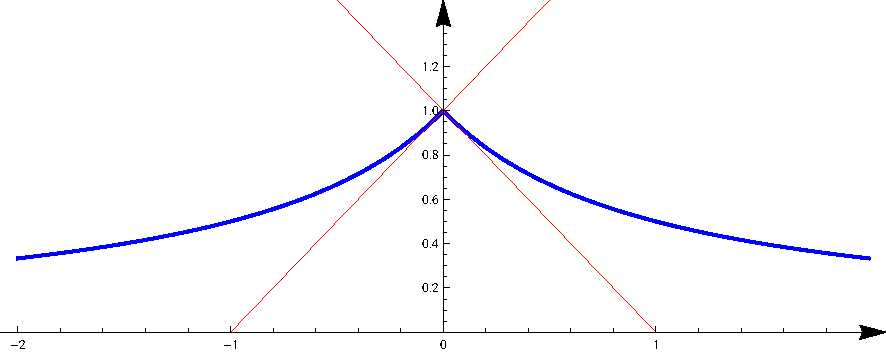
\includegraphics[scale=0.4]{abs.pdf}
\end{center}
\end{block}
\end{frame}

\begin{frame}{Примеры}
\begin{block}{Бесконечная производная}
Бесконечная производная функции в точке означает существование вертикальной касательной в этой точке. Например, пусть 
$$f(x)=\left\{ \begin{array}{cl}
\sqrt[3]{x},& x\ge0;\\
-\sqrt[3]{|x|},& x<0.
\end{array}\right.
$$
Тогда, очевидно, $f'(0) = +\infty$.
\end{block}
Теорема о производной обратной функции естественным образом распространяется на случай $f'(x_0) = 0$ или $\pm\infty$. Тогда $g'(y_0)$ равно $\pm\infty$ или $0$ соответственно, где $g$ --- обратная к $f$ функция.
\begin{block}{Пример недифференцируемой функции}
Рассмотрим $f(x) = x \sin(1/x)$ при $x\ne0$ и $f(0) = 0$. Тогда
$$f'(x) = x \cos(1/x)+\sin(1/x),\quad x\ne0.$$
Следовательно, у непрерывной функции $f(x)$ не существует даже односторонних касательных в точке $x=0$.
\end{block}
\end{frame}

\begin{frame}{Дифференциалы высших порядков}
\begin{block}{Определение}
Функция $f(x)$ называется является дважды дифференцируемой в точке $x_0$, если функция $f'(x)$  определена в окрестности  $x_0$ и дифференцируема в точке $x_0$. Вторая производная $f$ имеет вид
$$f''(x_0) = \left( f'(x) \right)'\Big|_{x=x_0}.$$
Аналогично определяются производные любого порядка.
\end{block}
Найдем второй дифференциал, учитывая, что функция $dx(h) = h$ не зависит от $x$, а зависит только от независимого приращения $h$:
$$d^2 f(x) = d\left( df(x) \right) = d\left( f'(x)dx\right) = f''(x)d^2x.$$
Для второй производной часто используют обозначения:
$$f''(x) = \frac{d^2 f(x)}{dx^2}.$$
\vskip-1em
\begin{block}{Утверждение}
Несложно доказать по индукции, что
$$\frac{d^n}{dx^n}\left( f(x) g(x) \right) = \sum_{k=0}^n C_n^k f^{(k)}(x) g^{(n-k)}(x).$$
\end{block}

\end{frame}

\begin{frame}{Дифференциалы высших порядков}
\begin{block}{Пример}
Рассмотрим многочлен степени $n$:
$$P(x) = a_n x^n + a_{n-1} x^{n-1}+\cdots+a_0.$$
Тогда
$$P(0) = a_0,$$
$$P'(0) = \left(n a_n x^{n-1}+\cdots+2 a_2 x+a_1\right)\Big|_{x=0} = a_1,$$
$$\cdots$$
$$P^{(k)}(0) = k! a_k,$$
$$\cdots$$
$$P^{(n)}(0) = n! a_n.$$
Следовательно, любой многочлен $P(x)$ степени $n$ можно представить в виде:
$$P(x) = P(0) + \frac{P'(0)}{1!}x+\cdots+\frac{P^{(k)}(0)}{k!}x^k+\cdots+\frac{P^{(n)}(0)}{n!}x^n = \sum_{k=0}^n \frac{P^{(k)}(0)}{k!}x^k.$$
\end{block}
\end{frame}

\begin{frame}{Функции, заданные неявно или параметрически}
\begin{block}{Неявно заданная функция}
Иногда значение функции $y(x)$ определяется не из явной формулы вида
$$y(x) = \ldots,$$
а из уравнения содержащего $x$ и $y$. В этом случае говорят, что функция {\bf задана неявно}. 
\end{block}
\begin{block}{Пример}
Уравнение окружности имеет вид:
$$y^2+x^2=r^2.$$
Поскольку каждому значению $x$ должно соответствовать только одно значение функции $y(x)$, рассмотрим верхнюю полуокружность $y>0$.
\vskip1em 
Если необходимо найти производную $y'(x)$ при $x_0=r\sqrt{2}/2$ и $y(x_0) =r\sqrt{2}/2$. Предполагая, что $y(x)$ дифференцируема в этой точке, получаем
$$2y'(x_0) y(x_0)+2x_0 =0\quad \Rightarrow\quad y'(x_0) = - \frac{x_0}{y(x_0)} = -1.$$
\end{block}

\end{frame}

\begin{frame}{Функции, заданные неявно или параметрически}
\begin{block}{Параметрически заданная функция}
Говорят, что функция задана параметрически, если
$$
\left\{ \begin{array}{l}
y=y(t);\\
x=x(t),
\end{array}
\right.
$$
где $t$ --- параметр. Пусть в окрестности $t=t_0$  существует функция $t=t(x)$, обратная к $x(t)$. Определим $Y(x)=y(t(x))$, $x_0=x(t_0)$. Если функции $y(t)$, $x(t)$ и $t(x)$ дифференцируемы, то производная $Y'(x_0)$ имеет вид:
$$Y'(x_0)=\frac{dy(t(x))}{dx}\Big|_{x=x_0}=y'(t(x_0))t'(x_0)=\frac{y'(t_0)}{x'(t_0)}.$$
Таким образом,
$$\frac{dY(x_0)}{dx}=\frac{y'(t_0)}{x'(t_0)}.$$
\end{block}
\end{frame}

\begin{frame}{Основные теоремы дифференциального исчисления. Теорема Ферма.}
\begin{block}{Лемма}
Пусть функция $f(x)$ дифференцируема в точке $x_0$. Тогда, если $f'(x_0)>0$ ($f'(x_0)<0$), то функция $f(x)$ возрастает (убывает) в некоторой окрестности $x_0$.
\end{block}
Доказательство следует непосредственно из определения производной и свойств предела (свойство сохранения знака).
\begin{block}{Теорема Ферма}
Пусть функция $f(x)$ определена на интервале $(a,\,b)$ и принимает наибольшие или наименьшее значение в точке $x_0\in(a,b)$. Тогда, если функция $f(x)$ дифференцируема в $x_0$, то необходимо $f'(x_0)=0$.
\end{block}
\begin{block}{Доказательство}
Предположим обратное. Тогда немедленно получаем противоречие с леммой.
\end{block}
\begin{block}{Упражнение}
Проведите самостоятельно полное подробное доказательство леммы и теоремы Ферма.
\end{block}
\end{frame}

\begin{frame}{Основные теоремы дифференциального исчисления. Теорема Ферма.}
\begin{block}{Определение}
Точка $x_0$ называется точкой локального максимума (минимума) функции $f(x)$, а значение $f(x_0)$ называют локальным максимумом (минимумом) функции $f(x)$, если $f(x_0)$ является максимумом (минимумом) значений функции $f(x)$ для $x$ из некоторой окрестности точки~$x_0$.
\vskip1em
Аналогично формулируется определение для точек строгого максимума и минимума.
\end{block}
Например, $x_0$ --- точка локального минимума $f(x)$, если существует окрестность $U$ точки $x_0$ такая, что
$$f(x_0)\le f(x) \qquad \forall x\in U.$$
Точки локального максимума и минимума вместе называют точками локального экстремума функции.

\begin{block}{Геометрический смысл теоремы Ферма}
Касательная, если она существует,  является горизонтальной в точках локального экстремума функции $f(x)$.
\end{block} 
\end{frame}

\begin{frame}{Основные теоремы дифференциального исчисления. Теорема Ферма.}
\begin{block}{Алгоритм поиска максимума функции на отрезке}
Пусть $f(x)$ непрерывна на отрезке $[a,b]$. Тогда, по теореме Вейерштрасса она достигает своего минимального и максимального значения на этом отрезке. Из теоремы Ферма следует, что для поиска точек глобального минимума и максимума функции $f(x)$ необходимо рассмотреть:
\begin{enumerate}
\item Все точки интервала $(a,b)$, для которых $f'(x)=0$.
\item Все точки интервала $(a,b)$, в которых не существует $f'(x)$.
\item Граничные точки $x=a$ и $x=b$.
\end{enumerate}
Глобальный максимум и минимум $f(x)$ обязательно достигается в одной (или в нескольких) из этих точек.
\end{block} 
\begin{block}{Пример}
Пусть $f(x)=e^x-x-1$ при $x\in\mathbb{R}$. Тогда
$$f'(x) =e^x -1=0\quad \Leftrightarrow \quad x=0.$$
Учитывая, что $f(x)\to+\infty$ при $x\to\infty$, получаем, что $\min f(x) = f(0)=0$, $\sup f(x) =+\infty$.
Следовательно, справедливо неравенство:
$$e^x\ge 1+x \qquad \forall x\in\mathbb{R}.$$
\end{block}
\end{frame}

\begin{frame}{Основные теоремы дифференциального исчисления. Теорема Роля.}
\begin{block}{Теорема Ролля}
Пусть $f(x)$ непрерывна на отрезке $[a,b]$ и дифференцируема на интервале $(a,b)$. Тогда, если $f(a)=f(b)$, то существует точка $c\in(a,b)$ такая, что $f'(c)=0$.
\end{block} 
\begin{block}{Доказательство}
По второй теореме Вейерштрасса существует $x_{min}$ и $x_{max}$ такие, что
$$f(x_{min}) = m=\min_{x\in[a,b]} f(x),\qquad f(x_{max}) = M= \max_{x\in[a,b]} f(x).$$
Возможны два случая
\begin{enumerate}
\item Если $m=M$, то функция $f(x)=m$ при всех $x\in(a,b)$. Тогда в качестве точки $c$ можно взять любую точку из интервала $(a,b)$.
\item Если $m<M$, то $m\ne f(a)$ или $M\ne f(a)$. Следовательно, одна из точек $x_{min}$ или $x_{max}$ заведомо лежит на интервале $(a,b)$, а не совпадает с точками $a$ и $b$. Пусть $c$ --- эта точка, то есть $x_{min}$ или $x_{max}$. Тогда по теореме Ферма $f'(c)=0$.
\end{enumerate}
\end{block}
\end{frame}

\begin{frame}{Основные теоремы дифференциального исчисления. Теорема Ролля.}
\begin{block}{Геометрический смысл теоремы Ролля}
Если дифференцируемая функция принимает равные значения на концах интервала, то найдется точка на интервале такая, что касательная в этой точке будет горизонтальной.
\end{block} 
\begin{center}
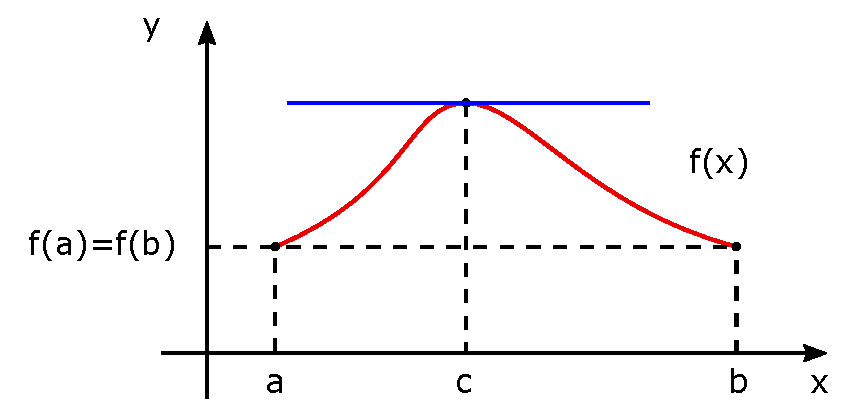
\includegraphics[scale=0.5]{thRolly.pdf}
\end{center}
\begin{block}{Физический смысл теоремы Ролля}
Если точка движется по прямой и в какой-то момент времени оказывается в начальной точке, то обязательно в некоторой момент времени точка совершила поворот в направление своего движения, то есть в некоторый момент времени скорость точки была равна $0$. 
\end{block} 
\end{frame}

\begin{frame}{Основные теоремы дифференциального исчисления. Теорема Лагранжа.}
\begin{block}{Теорема Лагранжа}
Пусть $f(x)$ непрерывна на отрезке $[a,b]$ и дифференцируема на интервале $(a,b)$. Тогда существует точка $c\in(a,b)$ такая, что
$$f(b)-f(a) = f'(c)(b-a).$$
Данную формулу называют формулой Лагранжа или формулой конечных приращений.
\end{block} 
\begin{block}{Доказательство}
Рассмотрим функцию 
$$g(x)=f(x)-(x-a)\frac{f(b)-f(a)}{b-a}.$$
Функция $g(x)$ удовлетворяет всем требованиям теоремы Ролля, так как $g(a)=g(b)=f(a)$. Следовательно, существует $c\in(a,b)$ такая, что $g'(c)=0$. Получаем
$$g'(x) = f'(x) - \frac{f(b)-f(a)}{b-a}\quad \Rightarrow \quad f'(c) = \frac{f(b)-f(a)}{b-a},$$
что и требовалось доказать.
\end{block}
\end{frame}

\begin{frame}{Основные теоремы дифференциального исчисления. Теорема Лагранжа.}
\begin{block}{Геометрический смысл теоремы Лагранжа}
Если функция дифференцируема на интервале, то существует точка, в которой касательная параллельна хорде, которая соединяет значения функции на концах заданного интервала.
\end{block} 
\begin{columns}[T, onlytextwidth]
\begin{column}{0.55\textwidth}
	\only<2>{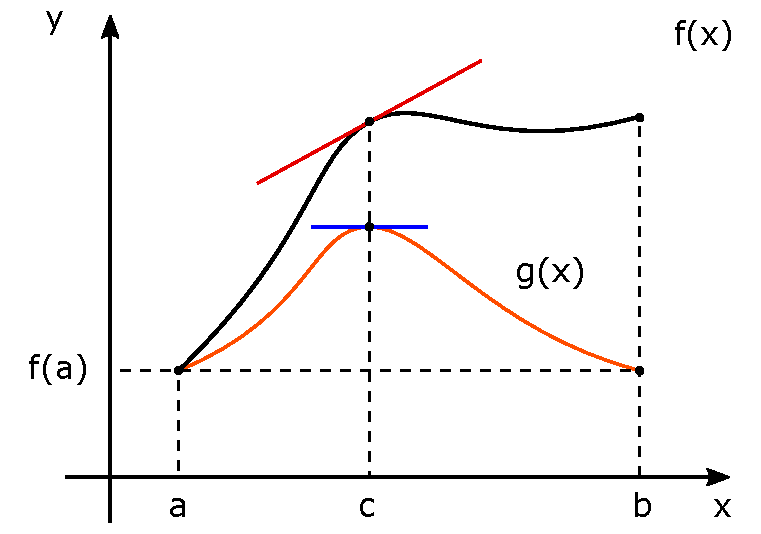
\includegraphics[scale=0.5]{thLagr0.pdf}}
	\only<1>{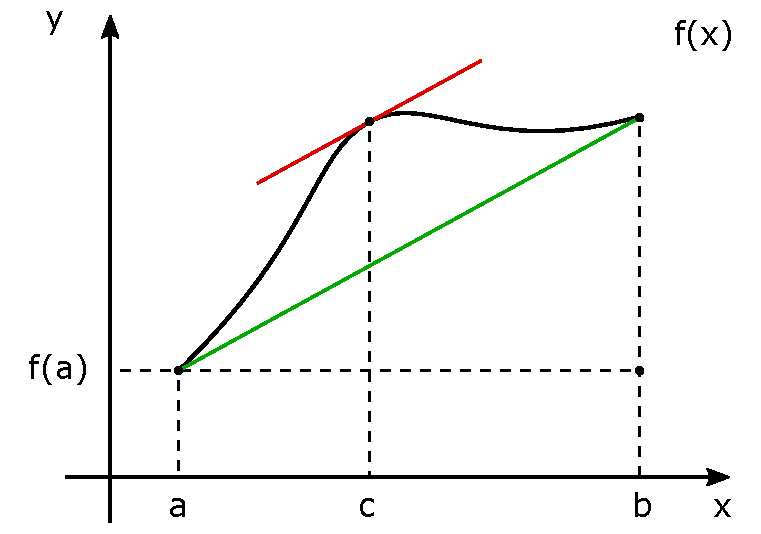
\includegraphics[scale=0.5]{thLagr.pdf}}
\end{column}
\begin{column}{0.45\textwidth}
	Формула Лагранжа:
	$$f(b)-f(a) = f'(c)(b-a).$$
	Уравнение хорды:
	$$y_{\text{хорд.}} = f(a)+(x-a)\frac{f(b)-f(a)}{b-a}.$$
	\only<2>{
		Формула для $g(x)$:
		$$g(x)=f(x)-(x-a)\frac{f(b)-f(a)}{b-a}.$$
	}
\end{column}
\end{columns}
\end{frame}

\begin{frame}{Теорема Лагранжа. Замечания}
\begin{block}{Физический смысл теоремы Лагранжа}
Пусть точка движется по прямой с переменной скоростью в течение определенного интервала времени. Тогда в некоторый момент времени мгновенная скорость точки в точности совпадала со средней скоростью на этом интервале.
\end{block}
\begin{block}{Замечания}
\begin{enumerate}
\item Теорему Лагранжа иногда называют теоремой о среднем значении в дифференциальном исчислении.
\item Теорема Ролля является частным случаем теоремы Лагранжа. Действительно, если $f(a)=f(b)$, то
$$0=f(b)-f(a) = f'(c)(b-a) \quad \Rightarrow \quad f'(c) = 0.$$
\item Формула конечных приращений Лагранжа сохраняет силу и при $b\le a$, если точки $a$ и $b$ взяты из интервала, на котором функция $f(x)$ дифференцируема. Точка $c$, очевидно, зависит от выбора точек $a$ и $b$.
\item Пусть $f(x)$ дифференцируема в окрестности точки $x_0$ и приращение $\Delta x$ координаты $x$ не выводит из этого интервала. Тогда формулу Лагранжа можно переписать в виде
$$\Delta f(x_0) = f(x_0+\Delta x) - f(x_0) = f'(x_0+\theta \Delta x)\,\Delta x,\quad \theta\in(0,1),$$
где $c=x_0+\theta\, \Delta x$.
\end{enumerate}
\end{block} 
\end{frame}

\begin{frame}{Теорема Лагранжа. Следствия}
\begin{block}{Теорема (Признак монотонности функции)}
Если функция дифференцируема на некотором интервале, то она строго возрастает (строго убывает) на нем тогда и только тогда, когда ее производная на этом интервале положительна (отрицательна).
\vskip1em
Очевидно, это утверждение справедливо и для случая нестрогой монотонности и не отрицательной (не положительной) производной.
\end{block}

\begin{block}{Теорема (Признак постоянства функции)}
Если функция дифференцируема на некотором интервале и ее производная тождественно равна $0$, то эта функция является постоянной на данном интервале.
\end{block}

\begin{block}{Пример}
Рассмотрим $f(x) = \arctg(x)+\arctg(1/x)$. Тогда
$$f'(x) = \frac{1}{x^2+1} + \frac{1}{1+(1/x)^2}\,\frac{-1}{x^2} \equiv 0,\quad \forall x>0 \quad \Rightarrow \quad f(x) \equiv f(1)=\frac{\pi}{4}+\frac{\pi}{4} = \frac{\pi}{2} .$$
Аналогично, $f(x)\equiv -\pi/2$ при $x<0$.
\end{block}

\end{frame}

\begin{frame}{Теорема Коши.}
\begin{block}{Теорема Коши}
Пусть $x(t)$ и $y(t)$ непрерывны на отрезке $[\alpha,\beta]$ и дифференцируемы на интервале $(\alpha,\beta)$, $x'(t)\ne0$ при $t\in(\alpha,\beta)$. Тогда существует точка $\xi\in(\alpha,\beta)$ такая, что
$$\frac{y(\beta)-y(\alpha)}{x(\beta)-x(\alpha)} = \frac{y'(\xi)}{x'(\xi)}.$$
Данную формулу называют формулой конечных приращений Коши.
\end{block} 
Формула Коши является аналогом формулы Лагранжа для функций, заданных параметрически. Из условий теоремы следует, что функция $x(t)$ строго монотонна. Тогда $x(\alpha)\ne x(\beta)$ и существует монотонная функция $t=t(x)$, обратная к $x=x(t)$ при $t\in(\alpha,\beta)$. 
\begin{block}{Упражнение}
Докажите теорему Коши, применяя формулу Лагранжа к функции $Y(x)=y(t(x))$.
\end{block}
Если просто применить формулу Лагранжа к $x(t)$ и $y(t)$ в отдельности, то получим
$$\frac{y(\beta)-y(\alpha)}{x(\beta)-x(\alpha)} = \frac{y'(\xi_1)(\beta-\alpha)}{x'(\xi_2)(\beta-\alpha)}=\frac{y'(\xi_1)}{x'(\xi_2)}.$$
Суть формулы Коши в том, что $\xi_1$ и $\xi_2$ можно выбрать равными!
\end{frame}

\begin{frame}{Формула линеаризации}
Задача состоит в построении наилучшего линейного приближения для функции $f(x)$ в окрестности точки $x_0$.
\begin{block}{Формула линеаризации}
Если функция $f(x)$ дифференцируема в точке $x_0$, то
$$f(x)=f(x_0)+f'(x_0)(x-x_0)+o(x-x_0).$$
Ограничиваясь только линейной частью, получаем приближенную формулу
$$f(x)\approx f(x_0)+f'(x_0)(x-x_0).$$
Эту формулу называют {\bf формулой линеаризации}. Заметим, что график линейной части в приближении функции $f(x)$ --- это касательная в точке $x_0$.
\end{block}
Формула линеаризации дает наилучшее линейное приближение функции $f(x)$ при $x\to x_0$.
\begin{block}{Пример}
Пусть $f(x) = \ln(\cos(x)+x)$, $x_0=0$. Тогда:
$$f(0) = 0,\quad f'(0)  =\frac{1-\sin(x)}{\cos(x)+x}\Big|_{x=0} = 1
\quad\Rightarrow\quad 
f(x) = x + o(x)\quad (x\to0).$$
\end{block} 
\end{frame}

\begin{frame}{Многочлен Тейлора}
Построим нелинейное приближение функции $f(x)$ в окрестности $x_0$ при помощи многочлена произвольной степени. 

\begin{block}{Предложение (о многочлене Тейлора)}
Пусть функция $f(x)$ дифференцируема $n$ раз в $x_0$, а $P(x)$ --- многочлен степени $n$. Тогда значения первых $n$ производных $f$ и $P$ совпадают в точке $x_0$:
$$f^{(k)}(x_0) = P^{(k)}(x_0),\quad (k=0,1,\ldots,n)$$
тогда и только тогда, когда
$$P(x)  = f(x_0) + \frac{f'(x_0)}{1!}(x-x_0) + \cdots + \frac{f^{(n)}(x_0)}{n!}(x-x_0)^n.$$
Многочлен $P(x)$ называют {\bf многочленом Тейлора} степени $n$ функции $f(x)$ в точке $x_0$.
\end{block}
\begin{block}{Доказательство}
Несложно получить (формула Тейлора для многочленов), что
$$P(x) =  P(x_0) + \frac{P'(x_0)}{1!}(x-x_0) + \cdots + \frac{P^{(n)}(x_0)}{n!}(x-x_0)^n,$$
для любого многочлена $P(x)$. Дальнейшее доказательство проведите самостоятельно.
\end{block}
\end{frame}

\begin{frame}{Многочлен Тейлора}
Мы предполагаем, что многочлен $P(x)$ является хорошим приближением для функции $f(x)$ в окрестности точки $x_0$, поскольку совпадают не только значения $f(x_0)$ и $P(x_0)$ но и все производные до $n$-го порядка включительно. 
\begin{block}{Определение}
Величину
$$r(x) = r_n(x, x_0)  = f(x)  - P(x),$$
где $P(x)$ --- многочлен Тейлора порядка $n$ в точке $x_0$, называют {\bf остаточным членом} порядка~$n$.
\end{block}
Следовательно, справедлива формула
$$f(x) =  f(x_0) + \frac{f'(x_0)}{1!}(x-x_0) + \cdots + \frac{f^{(n)}(x_0)}{n!}(x-x_0)^n + r_n(x).$$
Эту формулу называют {\bf формулой Тейлора}.
\begin{block}{Пример}
Пусть $f(x) = e^x$, $x_0 = 0$. Тогда
$$f^{(n)}(x) = e^x,\quad \Rightarrow\quad f^{(n)}(0) = 1\quad \Rightarrow\quad$$
$$e^x  =1+ \frac{x}{1!} + \frac{x^2}{2!} + \cdots + \frac{x^n}{n!}+r_n(x).$$
\end{block}
\end{frame}

\begin{frame}{Многочлен Тейлора. Формула Пеано}
\begin{block}{Лемма}
Пусть функция $g(x)$ дифференцируема $n$ раз в точке $x_0$ и 
$$g(x_0) = g'(x_0) = \ldots = g^{(n)}(x_0) = 0.$$
Тогда $g(x)  = o((x-x_0)^n)$.
\end{block}
\begin{block}{Доказательство}
Данная лемма справедлива для $n=1$:
$$g(x)  = g(x_0) + g'(x_0) ( x - x_0) +o(x-x_0) = o(x-x_0), \quad (x\to x_0).$$
Пусть она справедлива для $n-1$. Тогда, применяя ее к $g'(x)$, получаем
$$g'(x)  = o(x-x_0)^{n-1} = \alpha(x) (x-x_0)^{n-1}, \quad (x\to x_0),$$
где $\alpha(x)$ --- бесконечно малая функция.
Применяя формулу конечных приращений $g(x) = g'(\xi)(x - x_0)$, получаем
$$\left| g(x) \right|= \left|g'(\xi)(x - x_0)\right| =
\left| \alpha(\xi) (\xi-x_0)^{n-1}(x - x_0) \right|\le 
| \alpha(\xi)|\, |(x-x_0)^{n}|.$$
Следовательно, $g(x) =  o(x-x_0)^n$.
\end{block}

\end{frame}

\begin{frame}{Многочлен Тейлора. Формула Пеано}
Остаточный член $r_n(x)$ удовлетворяет всем требованиям предыдущей леммы. Следовательно, справедлива следующая теорема.
\begin{block}{Теорема. Формула Тейлора с остаточным членом в форме Пеано}
Пусть функция $f(x)$ дифференцируема $n$ раз в точке $x_0$.
Тогда 
$$f(x) =  f(x_0) + \frac{f'(x_0)}{1!}(x-x_0) + \cdots + \frac{f^{(n)}(x_0)}{n!}(x-x_0)^n +o(x-x_0)^n\quad (x\to x_0).$$
\end{block}
В случае $n=1$ получаем формулу из определения дифференцируемости функции
$$f(x) - f(x_0) = f'(x_0) (x - x_0) + o(x-x_0).$$
При $x_0= 0 $ формулу Тейлора
$$f(x) =  f(0) + \frac{f'(0)}{1!}x + \cdots + \frac{f^{(n)}(0)}{n!}x^n +o(x^n)\quad (x\to 0),$$
часто называют формулой Маклорена.
\vskip1em
Таким образом, формула Тейлора может быть использована для построения хороших приближенных формул с малой погрешностью порядка $o(x-x_0)^n$.
\end{frame}

\begin{frame}{Многочлен Тейлора. Примеры}

\begin{block}{Синус и косинус}
Рассмотрим $f(x)=\sin(x)$, $x_0 = 0$. Тогда:
$$
f'(0) = \cos(x)\Big|_{x=0} = 1,\quad
f''(0) = -\sin(x)\Big|_{x=0} = 0,\quad
f^{(3)}(0) = -\cos(x)\Big|_{x=0} = -1,\quad\ldots
$$
$$\sin(x) = x - \frac{x^3}{3!}+\frac{x^5}{5!}-\cdots+(-1)^n \frac{x^{2n+1}}{(2n+1)!}+o(x^{2n+1}).$$
Аналогично,
$$\cos(x) = 1 - \frac{x^2}{2!}+\frac{x^4}{4!}-\cdots+(-1)^n \frac{x^{2n}}{(2n)!}+o(x^{2n}).$$
\end{block}
\vskip-1em
\begin{block}{Логарифм}
Рассмотрим $f(x) = \ln(1+x)$, $x_0 = 0$. Тогда
$$f'(x) = \frac{1}{1+x} \quad\Rightarrow\quad 
f^{(n)}(x) = \frac{(-1)^{n-1}(n-1)!}{(1+x)^n}\quad\Rightarrow\quad $$
$$\ln(1+x) =x-\frac{x^2}{2}+\frac{x^3}{3}-\cdots+(-1)^{n-1}\frac{x^n}{n}+o(x^n).$$
\end{block}
\end{frame}

\begin{frame}{Многочлен Тейлора. Примеры}
\begin{block}{Степенная функция}
Рассмотрим $f(x)=(1+x)^\alpha$, $x_0 = 0$. Вычисляя производные, получаем
$$
f'(0) = \alpha(1+x)^{\alpha-1}\Big|_{x=0} = \alpha,\quad
f''(0) =\alpha(\alpha-1)(1+x)^{\alpha-2}\Big|_{x=0} = \alpha(\alpha-1),\quad \ldots
$$
$$(1+x)^\alpha= 1+\alpha x+\frac{\alpha(\alpha-1)}{2!}x^2+\cdots+\frac{\alpha(\alpha-1)\cdots (\alpha-n+1)}{n!} x^n+o(x^{n}).$$
Например:
$$\frac{1}{1+x}= 1- x+x^2-x^3+\cdots+(-1)^{n} x^n+o(x^{n}).$$
Поскольку это сумма геометрической прогрессии мы можем получить явную формулу для остатка $r_n(x)$:
$$ 1- x++\cdots+(-1)^{n} x^n = \frac{1-(-x)^{n+1}}{1-(-x)} = \frac{1}{1+x} - \frac{(-1)^{n+1}x^{n+1}}{1+x}\quad \Rightarrow$$
$$r_n(x) = \frac{1}{1+x} - \sum_{k=0}^n (-1)^k x^k= \frac{(-1)^{n+1}x^{n+1}}{1+x} = o(x^n).$$
\end{block}
\end{frame}

\begin{frame}{Многочлен Тейлора. Свойства}
Многочлен Тейлора дает наилучшее приближение для функции $f(x)$ в окрестности $x_0$.
\begin{block}{Предложение}
Пусть $f(x)$ дифференцируема n раз в точке $x_0$ и справедливо равенство
$$f(x) - P(x) = o(x-x_0)^n,\quad (x\to x_0),$$
где $P(x)$ --- многочлен степени $n$. Тогда $P(x)$ --- многочлен Тейлора.
\end{block}
\begin{block}{Доказательство}
Используя формулу Тейлора для многочлена $P(x)$ и функции $f(x)$, получаем тождество:
$$ f(x) - P(x) = \sum_{k=0}^n \frac{f^{(k)}(x_0)}{k!}(x-x_0)^k + o(x-x_0)^n-\sum_{k=0}^n \frac{P^{(k)}(x_0)}{k!}(x-x_0)^k,$$
$$f(x) - P(x) = o(x-x_0)^n\quad\Rightarrow\quad 
 \sum_{k=0}^n \frac{(f^{(k)}(x_0)-P^{(k)}(x_0))}{k!}(x-x_0)^k  = o(x-x_0)^n.$$
Подставляя $x=x_0$, получаем $P(x_0) = f(x_0)$. Далее, деля на $x-x_0$ и подставляя $x=x_0$, получаем $P'(x_0) = f'(x_0)$, и так далее.
\end{block}

\end{frame}

\begin{frame}{Многочлен Тейлора. Пример}
\begin{block}{Пример}
Рассмотрим функцию $\displaystyle f(x) = \frac{1}{1-x^2}$ при $x_0 = 0$
Вместо вычисления производных $f(x)$ можно воспользоваться уже известной формулой
$$\frac{1}{1+z} = 1-z+z^2-\cdots+(-1)^n z^n+o(z^n),$$
для $z=-x^2$. Тогда
$$\frac{1}{1-x^2} =1+x^2+x^4+\cdots+ x^{2n}+o(x^{2n}).$$
Из доказанного предложения следует, что $1+x^2+x^4+\cdots+ x^{2n}$ является многочленом Тейлора функции $f(x)$ и
$$f^{(2n+1)}(0)=0,\quad f^{(2n)}(0)=(2n)! \qquad \forall n\ge0.$$
Таким образом, мы нашли значения производных функции $f(x)$ вычисляя ее многочлен Тейлора.
\end{block}
\end{frame}

\begin{frame}{Многочлен Тейлора. Пример}
\begin{block}{Пример}
Найдем многочлен Тейлора для $f(x) = \arctg(x)$ при $x_0=0$. Получаем, что
$$f'(x) =g(x) =\frac{1}{1+x^2} = 1-x^2+x^4-\cdots+(-1)^n x^{2n}+o(x^{2n}).$$
Следовательно,
$$f^{(2n+2)}(0) = g^{(2n+1)}(0) = 0,\quad f^{(2n+1)}(0) = g^{(2n)}(0) = (-1)^n\, (2n)!\qquad \forall n\ge0.$$
Таким образом,
$$\arctg(x) =x-\frac{x^3}{3}+\frac{x^5}{5}+\cdots+(-1)^n\frac{x^{2n+1}}{2n+1}+o(x^{2n+1}).
$$
\end{block}
\begin{block}{Упражнение}
Аналогичным образом получите формулу:
$$\arcsin(x) = \sum_{k=0}^n  \frac{C_{2k}^k}{4^{k} (2k+1)}\, x^{2k+1}+o(x^{2n+1}).$$
\end{block}
\end{frame}

\begin{frame}{Многочлен Тейлора. Пример}

\begin{block}{Пример}
Найдем несколько первых членов в формуле Тейлора для $f(x) = \tg(x)$. Используя разложение для синуса, косинуса и формулу:
$$\frac1{1-z} = 1+z+z^2+o(z^2)\quad (z\to0),$$
получаем, что
$$\frac{1}{\cos(x)} =  \left(1-\frac{x^2}{2!}+o(x^3)\right)^{-1} = \left(1-\frac{x^2}{2}\left(1+o(x)\right)\right)^{-1}=1+\frac{x^2}{2}\left(1+o(x)\right)+o(x^3),$$
$$\tg(x) =\frac{\sin(x)}{\cos(x)}=
\left(x - \frac{x^3}{6}+o(x^4)\right)
\left(1+\frac{x^2}{2}+o(x^3)
\right)=x+\left(\frac12 - \frac16\right) x^3+o(x^4),$$
$$\tg(x)=x+\frac{x^3}{3}+o(x^4).$$
\end{block}
\vskip-1em
\begin{block}{Упражнение}
Проверьте этот результат, вычислив производные функции $f(x) = \tg(x)$.
\end{block}
\end{frame}

\begin{frame}{Многочлен Тейлора. Формула Лагранжа}
Формула Тейлора с остаточным членом в форме Пеано удобна для выяснения локальных свойств функции $f(x)$ при $x\to x_0$. С другой стороны, большой интерес представляет вопрос о явных оценках остаточного члена $r_n(x,x_0)$ в формуле Тейлора в случае конечного значения $x-x_0$.

\begin{block}{Теорема. Формула Лагранжа для остаточного члена}
Пусть функция $f(x)$ имеет производную порядка $n+1$ в окрестности точки $x_0$. Тогда для остаточного члена справедливы формулы Лагранжа:
$$r_n(x) = \frac{f^{(n+1)}(\xi)}{(n+1)!}(x-x_0)^{n+1},$$
где $x$ лежит в заданной окрестности $x_0$, а $\xi$ лежит между $x$ и $x_0$.  
\end{block}
Таким образом, справедлива формула
$$f(x) = f(x_0)+\frac{f'(x_0)}{1!}(x-x_0)+\cdots+\frac{f^{(n)}(x_0)}{n!}(x-x_0)^n+\frac{f^{(n+1)}(\xi)}{(n+1)!}(x-x_0)^{n+1}.$$
При $n=0$ получаем формулу конечных приращений Лагранжа:
$$f(x) = f(x_0) + f'(\xi)(x-x_0).$$
\end{frame}

\begin{frame}{Многочлен Тейлора. Формула Лагранжа}
\begin{block}{Доказательство}
По определению $\displaystyle r_n(x, x_0)= f(x) -P(x) =f(x) - \sum_{k=0}^n \frac{f^{(k)}(x_0)}{k!}(x-x_0)^k.$

Рассмотрим зависимость $r_n(x, x_0)$ от точки $x_0$. Для этого фиксируем точку $x$ и определим вспомогательную функцию
$$s(z) =  f(x) - \sum_{k=0}^n \frac{f^{(k)}(z)}{k!}(x-z)^k.$$
Функция $s(z)$ дифференцируема в окрестности точки $z=x_0$:
$$s'(z) = -\frac{d}{dz}\sum_{k=0}^n \frac{f^{(k)}(z)}{k!}(x-z)^k  = \frac{f^{(n+1)}(z)}{n!}(x-z)^n.$$
Пусть $u(z) = (x-z)^{n+1}$. Тогда, применяя формулу конечных приращений Коши к $s(z)$ и $u(z)$ на отрезке с концами $x$ и $x_0$, получаем, что
$$ \frac{s'(\xi)}{u'(\xi)}=\frac{s(x) - s(x_0)}{u(x) - u(x_0)} =
\frac{s(x_0)}{ u(x_0)}=\frac{r_n(x,x_0)}{(x-x_0)^{n+1}}\quad \Rightarrow \quad 
r_n(x,x_0)=\frac{f^{(n+1)}(\xi)}{(n+1)!}(x-x_0)^{n+1}.
$$
\end{block}
\end{frame}

\begin{frame}{Многочлен Тейлора. Пример}
\begin{block}{Другое определение числа $e$}
По формуле Тейлора с остаточным членом в форме Лагранжа получаем:
$$e^x= 1+\frac{x}{1!} + \frac{x^2}{2!}+\cdots+\frac{x^{n}}{n!}+r_n(x),\quad r_n(x)=e^{\xi}\frac{x^{n+1}}{(n+1)!}.$$
Следовательно,
$$e=1+\frac{1}{1!} + \frac{1}{2!}+\cdots+\frac{1}{n!}+r_n(1),$$
$$r_n(1)<\frac{e}{(n+1)!}\to 0 \quad (n\to+\infty).$$
Таким образом,
$$e = \lim_{n\to+\infty}\sum_{k=0}^n \frac{1}{k!} = 1+\frac{1}{1!} + \frac{1}{2!}+\cdots+\frac{1}{n!}+\ldots.$$
Заметим, что последовательность $\sum\limits_{k=0}^n \frac{1}{k!}$ сходится к $e$ значительно быстрее, чем последовательность $(1+1/n)^n$. Действительно,
$$\left(1+\frac{1}{n}\right)^n = e^{n\ln(1+1/n)}= e - \frac{e}{2n} + o\left(\frac{1}{n}\right).
 $$
\end{block}
\end{frame}

\begin{frame}{Исследование функций. Экстремум.}
По теореме Ферма производная функции обращается в ноль в точках локального экстремума. Следовательно, теорема Ферма дает необходимое условие для поиска экстремума. Построим достаточное условие.
\begin{block}{Теорема. Достаточное условие строгого локального экстремума}
Пусть функция $f(x)$ дифференцируема в окрестности точки $x_0$.
Точка $x_0$ является точкой строгого локального экстремума функции $f(x)$ тогда и только тогда, когда производная $f'(x)$ меняет знак в точке $x_0$. Если при этом $f'(x)$ меняет знак с минуса на плюс, то $x_0$ --- точка строго локального минимума, а иначе $x_0$ --- это точка максимума.
\end{block}
{\bf Доказательство} следует непосредственно из признака монотонности функции.
\begin{block}{Пример}
Пусть $f(x)=x^2$. Тогда $f'(x) = 2x$ и $f'(0) = 0$. Производная $f'(x)=2x$ меняет знак с минуса при $x<0$ на плюс при $x>0$, следовательно, $x=0$ --- точка минимума.
\end{block}
\begin{block}{Замечание}
Теорема справедлива и в том случае, когда производная $f'(x_0)$ не существует, но $f'(x)$ определена в некоторой проколотой окрестности точки $x_0$.
\end{block}
\end{frame}

\begin{frame}{Исследование функций. Экстремум.}
Иногда проверка знака производной в окрестности стационарной точки вызывает затруднения. Оказывается, определить является ли точка точкой экстремума можно, анализируя знаки старших производных.

\begin{block}{Теорема. Анализ знаков старших производных}
Пусть функция $f(x)$ дифференцируема $n$ раз в точке $x_0$ и
$$f'(x_0) = \ldots = f^{(n-1)}(x_0)=0,\quad f^{(n)}(x_0)\ne 0.$$
Тогда точка $x_0$ является точкой строгого локального минимума (максимума) функции $f(x)$ тогда и только тогда, когда $n$ - четно и $f^{(n)}(x_0)>0$ ($f^{(n)}(x_0)<0$).
\end{block}

\begin{block}{Доказательство}
Используем формулу Тейлора с остаточным членом Пеано:
$$f(x) - f(x_0) =\frac{ f^{(n)}(x_0)}{n!} (x-x_0)^n+o(x-x_0)^n = \frac{ f^{(n)}(x_0)+\alpha(x)}{n!} (x-x_0)^n,$$
где $\alpha(x)$ --- бесконечно малая функция при $x\to x_0$.
Следовательно, в некоторой проколотой окрестности точки $x_0$ приращение функции $f(x)$ меняет знак при нечетных $n$ и сохраняет знак при четных $n$. Если $n$ --- четное число, то знак приращения совпадает со знаком производной $f^{(n)}(x_0)$.
\end{block}
\end{frame}

\begin{frame}{Исследование функций. Экстремум.}
\begin{block}{Пример Коши}
Рассмотрим функцию
$$f(x) = \left\{
\begin{array}{ll}
e^{-1/x^2},& x\ne0;\\[.5em]
0,& x=0.
\end{array}\right.
$$
Несложно видеть, что $f(x)$ имеет производные любого порядка и 
$$f^{(n)}(0) = 0.$$
Таким образом, многочлен Тейлора функции $f$ равен тождественно $0$ и
$$f(x) = o(x^n),\quad (x\to0)\quad \forall n\in \mathbb{N}.$$
Очевидно, что точка $x=0$ является точкой глобального минимума функции $f$.
\end{block}
\begin{block}{Замечание}
Мы видели, что многочлены Тейлора однозначно определяются дифференцируемой функцией $f(x)$. Пример Коши показывает, что обратное утверждение не верно, поскольку функции $f(x)$ соответствуют те же многочлены Тейлора, что и у функции, тождественно равной нулю.
\end{block}
\end{frame}

\begin{frame}{Исследование функций. Выпуклость и вогнутость.}

\begin{block}{Определение}
Множество $E$ точек (на плоскости или в пространстве) называется {\bf выпуклым}, если вместе с любой парой точек $x$, $y$ из $E$ множеству $E$ принадлежит отрезок, соединяющий эти точки:
$$x\in E,\ y\in E \quad \Rightarrow \quad x+(y-x) t\in E \quad \forall t\in[0,1].$$
Иногда удобно вместо одного параметра $t$ рассмотреть два коэффициента $q_1$ и $q_2$:
$$x+(y-x) t=(1-t) x+t y=q_1 x+q_2 y\quad q_i\ge0,\ q_1+q_2=1.$$
Примерами выпуклых множеств являются выпуклые многоугольники и многогранники, шар, круг, т.д.
\end{block}
\begin{block}{Определение}
Функция $f(x)$ называется {\bf выпуклой} (выпуклой вниз) на промежутке от $a$ до $b$, если множество точек $(x,y)$, для которых $y\ge f(x)$, является выпуклым. Это множество называют {\bf надграфиком}.
\vskip1em
Аналогично, функция называется {\bf вогнутой} (выпуклой вверх), если множество точек, расположенных под графиком $f(x)$, является выпуклым.
\end{block}
\end{frame}

\begin{frame}{Исследование функций. Выпуклость и вогнутость.}
 Пусть функция $f(x)$ выпукла. Из определения выпуклости следует, что
 $$f(q_1 x_1+q_2 x_2)\le q_1 f(x_1)+q_2 f(x_2) ,\quad \forall q_i\ge0,\ q_1+q_2=1,\quad (\text{Неравенство Йенсена})$$
 где $x_1$ и $x_2$ --- точки из рассматриваемого промежутка. Верно и обратное утверждение, то есть из справедливости неравенства Йенсена для произвольных точек $x_{1,2}$ и коэффициентов $q_{1,2}$ следует выпуклость $f(x)$. Часто именно это неравенство выбирают за определение выпуклости.
 \begin{center}
 \only<1>{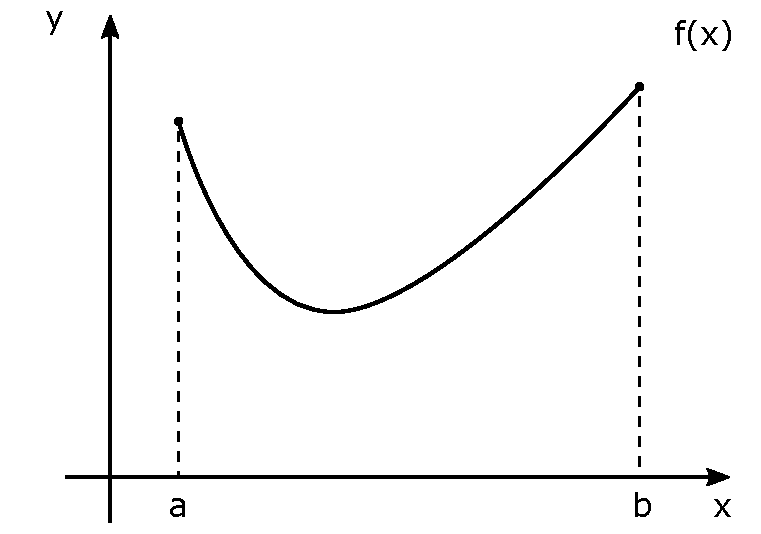
\includegraphics[scale=0.45]{vyp0.pdf}}
 \only<2>{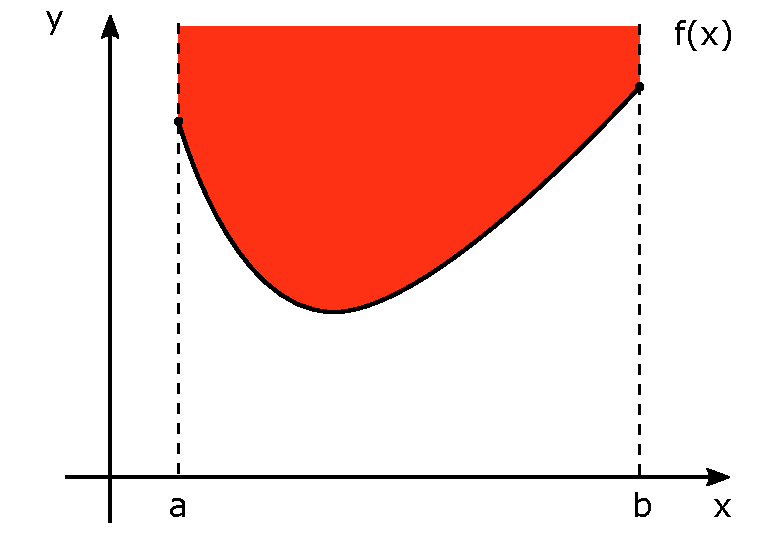
\includegraphics[scale=0.45]{vyp1.pdf}}
 \only<3>{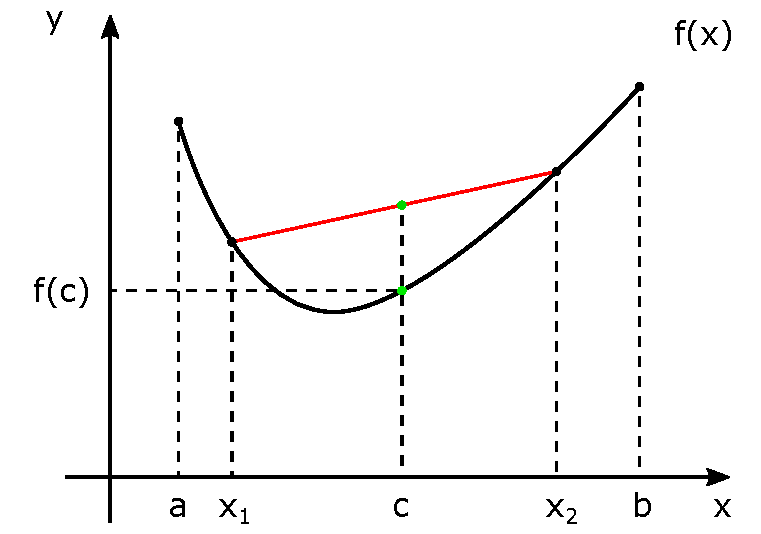
\includegraphics[scale=0.45]{vyp2.pdf}}
 \end{center}
Точка $c=q_1 x_1+q_2 x_2$,  $f(c)\le q_1 f(x_1)+q_2 f(x_2)$.
\end{frame}

\begin{frame}{Исследование функций. Выпуклость и вогнутость.}
Пусть функция $f(x)$ выпукла на отрезке $[a,b]$, а $x\in[a,b]$ --- произвольная точка. Тогда неравенство Йенсена можно переписать в виде:
$$f(x)\le \frac{x-a}{b-a} f(b) + \frac{b-x}{b-a} f(a),\quad \forall x\in[a,b],$$
или эквиваленто,
$$\frac{f(a) - f(x)}{a-x}\le \frac{f(b) - f(x)}{b-x},\quad \forall x\in[a,b].$$
\vskip-1em
\begin{block}{Теорема}
Пусть $f(x)$ дифференцируема на отрезке  $[a,b]$. Функция $f(x)$ является выпуклой тогда и только тогда, когда ее производная не убывает.
\end{block}
Если существует вторая производная, то $f''(x)\ge 0$ --- это условие выпуклости. 
\begin{block}{Следствие}
Все точки графика выпуклой функции лежат выше касательной к графику в произвольной точке.
\end{block}
\begin{block}{Упражнения}
Проведите последовательные доказательства утверждений, представленных на этом слайде, используя формулу конечных приращений. Сделайте соответствующие иллюстрации.
\end{block}
\end{frame}

\begin{frame}{Исследование функций. Асимптоты.}
\begin{block}{Определение}
Прямую $y=a x+b$ называют {\bf асимптотой} функции $f(x)$, если точки графика $f(x)$ стремятся к заданной прямой при $x\to \pm\infty$. В случае, если $f(x_0\pm0)\to\infty$, то говорят, что прямая $x=x_0$ --- вертикальная асимптота.
\end{block}
Несложно видеть, что $f(x)$ имеет наклонную асимптоту $y=a x+b$ при $x\to+\infty$ тогда и только тогда, когда
$$f(x) - (a x+b)\to0\quad (x\to+\infty).$$
Следовательно,
$$a = \lim_{x\to+\infty}\frac{f(x)}{x},\quad b = \lim_{x\to+\infty}\left(f(x) - a x\right).$$
Вычисляя эти пределы, можно проверить функцию на наличие наклонных асимптот.
\begin{block}{Пример}
Рассмотрим гиперболу $a y^2- b x^2= 1$, где $a>0$, $b>0$. Тогда
$$y(x) = \pm \frac{1}{\sqrt{a}} \sqrt{b x^2+1} = \pm x \sqrt{\frac{b}{a}}+o(x),\quad (x\to\infty).$$
 \end{block} 
\end{frame}

\begin{frame}{Правила Лопиталя}
Задача состоит в нахождении предела в случае неопределенности $\left(\frac{0}{0}\right)$.
\begin{block}{Теорема (Правило Лопиталя)}
Пусть выполнены условия:
\begin{enumerate}
\item функции $f(x)$ и $g(x)$ дифференцируемы в проколотой окрестности $x_0$ и производная $g'(x)\ne0$;
\item $f(x)\to0$, $g(x)\to0$ при $x\to x_0$;
\item существует (не обязательно конечный) предел отношения производных $f'(x)/g'(x)$ при~$x\to x_0$.
\end{enumerate}
Тогда существует предел отношения функций:
$$\lim_{x\to x_0} \frac{f(x)}{g(x)} = \lim_{x\to x_0} \frac{f'(x)}{g'(x)}.$$
\end{block}
\vskip-1em
\begin{block}{Доказательство}
Можно считать, что $f(x_0) = 0$ и $g(x_0) = 0$. Применяя формулу Коши, получаем:
$$\frac{f(x)}{g(x)} = \frac{f(x) - f(x_0)}{g(x)-g(x_0)} = \frac{f'(\xi)}{g'(\xi)}.$$
Далее достаточно применить теорему о пределе сложной функции, так как $\xi=\xi(x)\to x_0$~при $x\to x_0$ и $\xi(x)\ne x_0$.
\end{block}
\end{frame}

\begin{frame}{Правила Лопиталя}
Аналогичные правила справедливы и в случае бесконечного $x_0$, пределов справа и слева, и в случае неопределенностей вида $\left(\frac{\infty}{\infty}\right)$.
\begin{block}{Примеры}
Найдем пределы:
$$\lim_{x\to0} \frac{\sin(x)}{x} = \lim_{x\to0} \frac{\cos(x)}{1}=1.$$
$$\lim_{x\to +\infty} \frac{\ln(x)}{x} = \lim_{x\to +\infty} \frac{1/x}{1} =0.$$
$$\lim_{x\to +0} x\ln(x) = \lim_{x\to +0} \frac{\ln(x)}{1/x} = \lim_{x\to +0} \frac{1/x}{-1/x^2} = -\lim_{x\to +0} x = -0.$$
\end{block}
\vskip-1em
\begin{block}{Замечание}
В правилах Лопеталя условие существования предела отношения производных является необходимым условием. Бывает так, что предел отношения функций существует, а предел отношения производных --- нет. Например,
$$\lim_{x\to\infty}\frac{x+\sin(x)}{x}=1,\quad \lim_{x\to\infty}\frac{1+\cos(x)}{1}\ \text{ --- не существует.}$$
\end{block}
\end{frame}

\end{document}